\part{Create a Microservice}

\begin{frame}{Tomcat: Web Server and Servlet Container}
\begin{block}{Tomcat}
\begin{itemize}
\item Industry standard
\item Runs web applications
\item Small memory footprint
\end{itemize}
\end{block}

\vfill

\textbf{Why Tomcat}?
\begin{itemize}
\item Default in Cloud Foundry at SAP CP
\item Part of (SAP) Java Buildpack
\item Supported by SAP CP, no OS approval required
\end{itemize}

\vfill
Reference: \colorlink{https://github.wdf.sap.corp/cc-java-dev/cc-coursematerial/blob/master/_Internals/Tool_Decisions.md}{Tool Decisions}
\end{frame}


\begin{frame}[fragile]{Spring Web Application Components}
\begin{figure}
\includeGraphicsSpringWebApplicationComponents{width=\textwidth}
\end{figure}
\vfill
\scriptsize
\begin{itemize}
\item Servlet Filter - wraps servlet invocations
\item Dispatcher Servlet - dispatches web request to \codealt{Controller}
\item Handler Interceptor - allows to factor out pre- and postprocessing aspects of handlers
\item Exception Handler - maps message and HTTP status code
\item HTTPMessage Converter - converts Message to expected/supported \codealt{MediaType}
\end{itemize}
\end{frame}


\begin{frame}[fragile]{Spring Web Application Initialization}
\begin{lstlisting}[language=Java]
public class AppInitializer implements WebApplicationInitializer { 

    @Override
    public void onStartup(ServletContext servletContext) { // the "main" method"
        // register Spring Web servlet
        servletContext.addServlet("DispatcherServlet",
                new DispatcherServlet(applicationContext));	
        ...
        servletContext.addListener(new ContextLoaderListener(applicationContext));		
        servletContext.addFilter(...);  //Add Servlet Filter 
    }
}
\end{lstlisting}
\vfill
\codealt{WebApplicationInitializer} to configure the \codealt{ServletContext} with \ldots
\small
\begin{visibleenv}<2>
\begin{itemize}
\item \codealt{DispatcherServlet} - to dispatch web request to registered handlers
\item \codealt{ContextLoaderListener} - to load Java-based Spring Application Context
\item Servlet Filter - to wrap servlet invocations, e.g. authentication validation
\end{itemize}
\end{visibleenv}
\end{frame}


\begin{frame}{Exercise 1}
	\begin{figure}
		\includeGraphicsExerciseOne{width=0.8\textwidth}
	\end{figure}
 \colorlink{https://github.wdf.sap.corp/cc-java-dev/cc-coursematerial/blob/master/CreateMicroservice/Exercise_1_GettingStarted.md}{Exercise 1: Getting Started}
\end{frame}

\begin{frame}{RESTful Web Services}{Representational State Transfer}
A typical RESTful web service\ldots{}
\small
\begin{itemize}
\item provides a HTTP interface for a resource e.g. product
\item supports HTTP verbs: \codealt{POST}, \codealt{GET}, \codealt{PUT}, \codealt{PATCH}, \codealt{DELETE}
\item is stateless, scalable, cacheable
\item should be idempotent, i.e. multiple, identical requests behaves the same
\item provides atomic operations ("all or nothing") 
%compensation actions maybe required to bring the system into an consistent state, and MUST be documented
\end{itemize}
\vfill
\vspace{5mm}
\visible<2->{
\begin{tabular}{l|p{30mm}|p{30mm}}
\textbf{Endpoint} & \textbf{\codealt{GET}} & \textbf{\codealt{POST}} \\
\hline
\hline
\codealt{http://x/products} & query products (code 200) &  create new product (code 201) \\
\hline
\codealt{http://x/products/42} & show details of product (code 200) &  not supported (code 405) \\
\end{tabular}
\colorlink{http://www.restapitutorial.com/}{REST Tutorial}
\newline
\colorlink{http://www.restapitutorial.com/httpstatuscodes.html}{HTTP Status Codes}
}
\end{frame}


\begin{frame}{Guidance for Public REST APIs}
Harmonize HTTP-based APIs to improve consumption experience
\begin{itemize}
\item Unify conventions of plain REST and OData v4 APIs
\item General Guide \colorlink{https://jam4.sapjam.com/wiki/show/eBIJTH4EwfD15ymE2nv2pG}{CTO Whitepaper: "REST API Harmonization Direction"} (\colorlink{https://www.sap.com/documents/2017/12/ba1141bf-e37c-0010-82c7-eda71af511fa.html}{external link})
\end{itemize}
\vfill
\begin{block}{Plain REST vs. OData}
\small
\vspace{+1mm}
Consider OData, when \ldots
\begin{itemize}
  \item API is consumed by Fiori UIs
  \item You describe your HANA database model using CDS (XSA)
\end{itemize}
\end{block}
\vfill
Expose customer-facing API in the \colorlink{https://api.sap.com/}{SAP API Business Hub}
\end{frame}

\begin{frame}{What do HTTP Calls Look Like?}{Example: PUT Request}
\includeGraphicsPutRequestExplained{width=1.0\textwidth}
\vfill
\scriptsize \textbf{URL Formatting}\\
\begin{itemize} 
\item \codealt{https://<host>/<API namespace>/<API version>/<resource path>[?<query>]}
\item Example: \colorlink{}{https://api.sap.com/retail-store/v1/products/123}
\end{itemize}
\end{frame}


\begin{frame}[fragile]{Spring Web MVC: Building RESTful Services}
\textbf{Spring Web MVC} 
\small
\begin{itemize}
\item Is enabled / configured with \codealt{@EnableWebMvc}
\item Dispatches requests to \codealt{@Controller} annotated classes
\item  \colorlink{http://docs.spring.io/spring/docs/current/javadoc-api/org/springframework/web/bind/annotation/package-summary.html}{Convenient annotations}: \\\codealt{@RequestMapping}, \codealt{@GetMapping}, \codealt{@PathVariable}, \codealt{@RequestParam}, ...
\item Converts Java object $\Leftrightarrow$ JSON (using Jackson plugin)
\end{itemize}
\vfill
\begin{visibleenv}<2->
\vspace{-3mm}
\begin{block}{Example}
\begin{lstlisting}[language=Java,belowskip=-3mm,aboveskip=0mm]
@RequestMapping("products")
@RestController
public class ProductsController {

    @GetMapping(path = "/{id}")
    public Product getProduct(@PathVariable("id") long id) {
        return repository.findProduct(id);
    }
}
\end{lstlisting}
\end{block}
\end{visibleenv}
\end{frame}


\begin{frame}{Exercise 2}
	\begin{figure}
		\includeGraphicsExerciseTwo{width=0.8\textwidth}
	\end{figure}
 \colorlink{https://github.wdf.sap.corp/cc-java-dev/cc-coursematerial/blob/master/CreateMicroservice/Exercise_2_HelloWorldResource.md}{[Optional] Exercise 2: Provide Hello World Service on Tomcat}
\end{frame}



\begin{frame}{Domain: Bulletinboard - Advertisement Service}
 \begin{figure}
    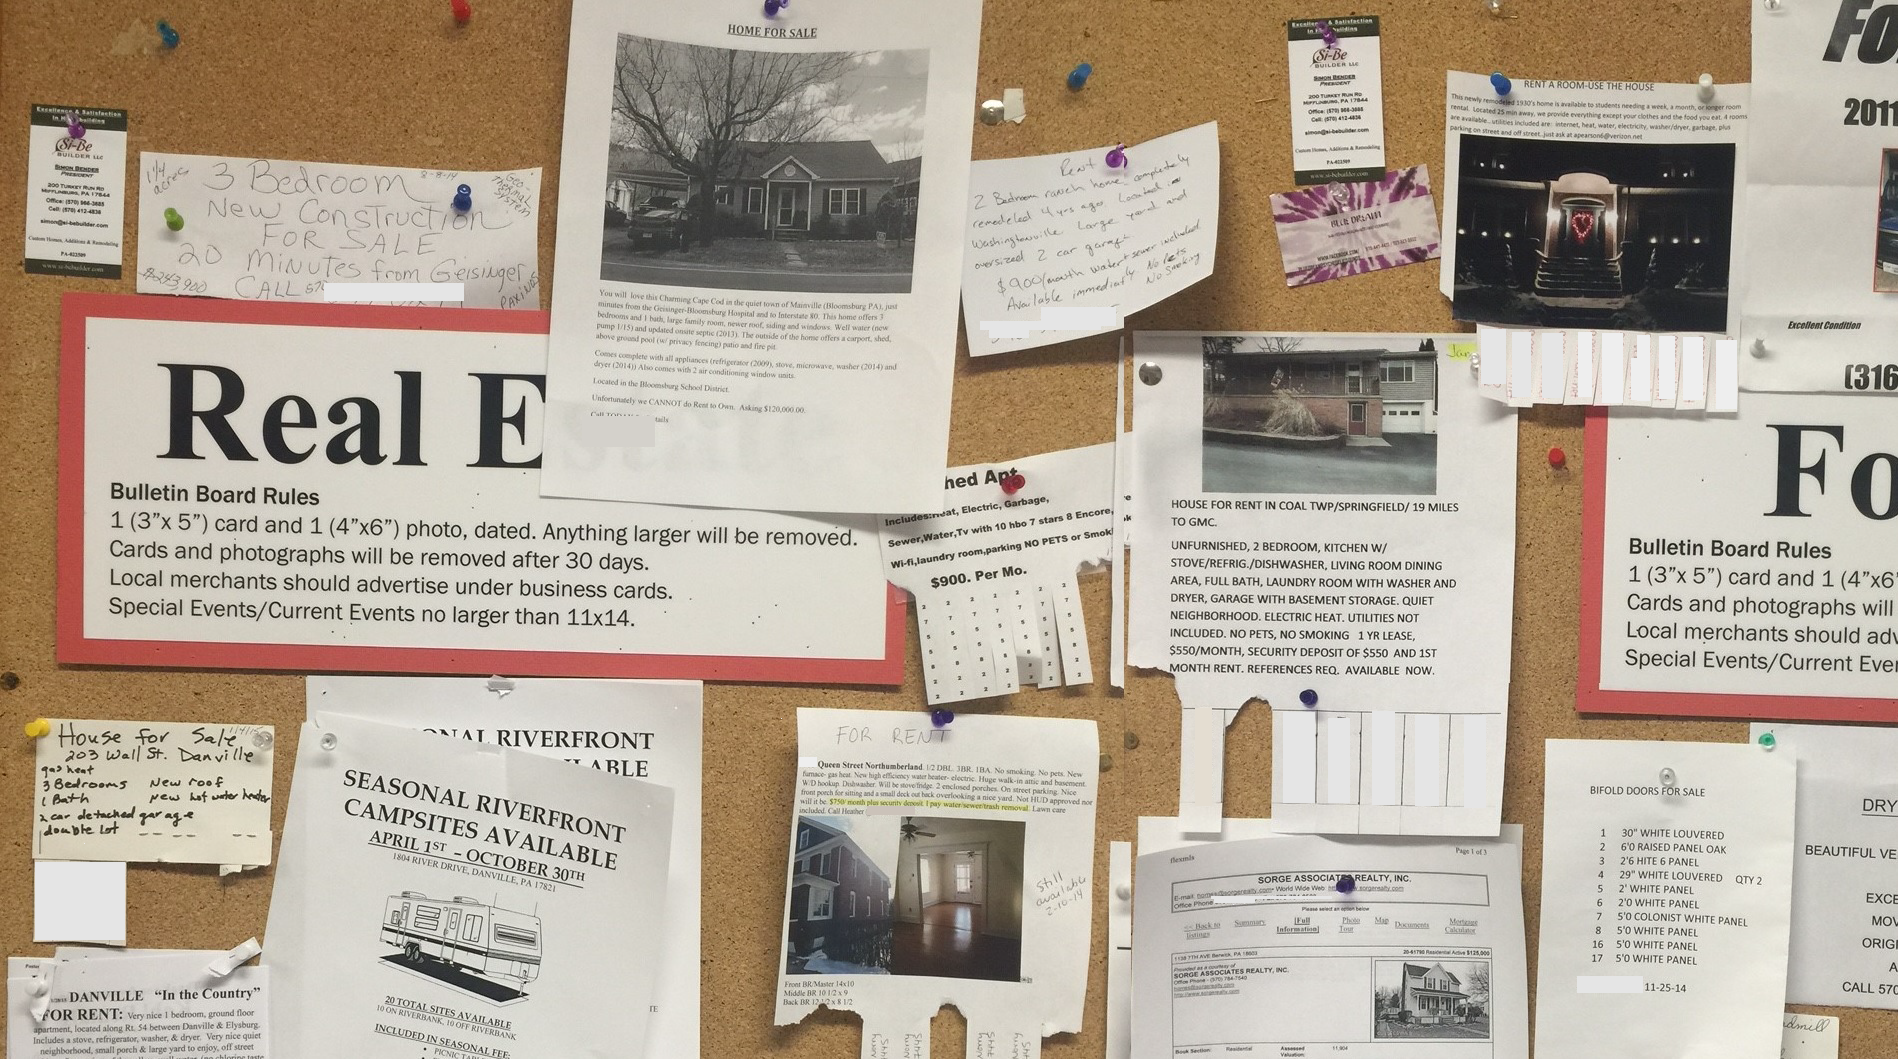
\includegraphics[width=\textwidth]{../CreateMicroservice//images/Bulletinboard}
  \end{figure}
\end{frame}

\begin{frame}{Domain: Bulletinboard - Advertisement Service}
\begin{figure}
	\includeGraphicsBigPicture{height=0.75\textheight}
\end{figure}
\end{frame}

\begin{frame}{Domain: Bulletinboard - Advertisement Service}
\begin{figure}
	\includeGraphicsBigPictureDetail{height=0.75\textheight}
\end{figure}
\end{frame}


\begin{frame}{Exercise 3}
	\begin{figure}
		\includeGraphicsExerciseThree{width=0.8\textwidth}
	\end{figure}
 \colorlink{https://github.wdf.sap.corp/cc-java-dev/cc-coursematerial/blob/master/CreateMicroservice/Exercise_3_CreateAdsEndpoints.md}{Exercise 3: Create Advertisement Endpoints}
\end{frame}


\begin{frame}[fragile]{Controller Test with Spring MVC Test}
\begin{itemize}
\small
\item Effective way for testing controllers: perform requests and generate responses through the actual \emph{DispatcherServlet}
\item No Servlet Container => fast feedback
\item \colorlink{https://docs.spring.io/spring/docs/current/spring-framework-reference/testing.html\#spring-mvc-test-vs-end-to-end-integration-tests}{Differences to End-to-End Integration Tests}
\end{itemize}
\vfill
\only<2>{
	\begin{figure}
	\includeGraphicsExerciseFour{height=0.6\textheight}
	\end{figure}
}
\begin{visibleenv}<3>
\begin{block}{Example: Test class}
\begin{lstlisting}[language=Java,belowskip=-3mm,aboveskip=0mm]
@RunWith(SpringJUnit4ClassRunner.class) // same to @RunWith(SpringRunner.class)
@ContextConfiguration(classes = { WebAppContextConfig.class })
@WebAppConfiguration
public class ControllerTest {
    private @Inject WebApplicationContext context; // reused for each test
    private MockMvc mockMvc;
    
    @Before
    public void setUp() throws Exception {
        this.mockMvc = MockMvcBuilders.webAppContextSetup(context)
		                       .addFilter(springSecurityFilterChain).build();
    }
}
\end{lstlisting}
\end{block}
\end{visibleenv}
\end{frame}

\begin{frame}[fragile]{Controller Test with Spring MVC Test}
\begin{block}{Example: Test case}
\begin{lstlisting}[language=Java,belowskip=-3mm,aboveskip=0mm]
import static org.sf.test.web.servlet.request.MockMvcRequestBuilders.*;
import static org.sf.test.web.servlet.result.MockMvcResultMatchers.*;

private MockMvc mockMvc;

@Test
public void readById() throws Exception {
   mockMvc.perform(buildGetRequest(id))
      .andExpect(status().isOk())
      .andExpect(content().contentType(APPLICATION_JSON_UTF8))
      .andExpect(jsonPath("$.title", is("buy me")));//com.jayway.jsonpath:json-path
}

private MockHttpServletRequestBuilder buildGetRequest(String id) throws Exception {
   return get("api/v1.0/ads/" + id).header(AUTHORIZATION, jwt);
}
\end{lstlisting}
\end{block}
\begin{itemize}
\item Use JUnit Test Framework/Runner
\item Use \codealt{Hamcrest} and \codealt{MockMvcResultMatchers} for readable assertions
\end{itemize}
\end{frame}

\begin{frame}[fragile]{Excursion: Spring MVC Test}
\begin{itemize}

	\item Build requests using the  \colorlink{http://docs.spring.io/spring/docs/current/javadoc-api/org/springframework/test/web/servlet/request/MockHttpServletRequestBuilder.html}{\codealt{MockHttpServletRequestBuilder}}
	\begin{lstlisting}
requestBuilder = post("path").content(jsonBody).contentType(APPLICATION_JSON);
	\end{lstlisting} 
	or
	\begin{lstlisting}
requestBuilder = get("path/" + id).header("Header", "Value");
	\end{lstlisting} 
\begin{visibleenv}<2->
	\item Invoke request, check and retrieve \colorlink{http://docs.spring.io/spring/docs/current/javadoc-api/org/springframework/mock/web/MockHttpServletResponse.html}{\codealt{MockHttpServletResponse}}
	\begin{lstlisting}
MockHttpServletResponse response = mockMvc.perform(requestBuilder)
            .andExpect(status().is2xxSuccessful())
            .andReturn().getResponse();
\end{lstlisting}
\end{visibleenv}
\begin{visibleenv}<3->
\item Create message content (JSON body):
	\begin{lstlisting}
String jsonBody = new ObjectMapper().writeValueAsString(anyObject);
	\end{lstlisting}
\end{visibleenv}
\end{itemize}
\end{frame}

\begin{frame}{Exercise 4}
	\begin{figure}
		\includeGraphicsExerciseFour{height=0.6\textheight}
	\end{figure}
 	\colorlink{https://github.wdf.sap.corp/cc-java-dev/cc-coursematerial/blob/master/CreateMicroservice/Exercise_4_CreateServiceTests.md}{Exercise 4: Create Automated Service Tests}
 	\colorlink{https://github.wdf.sap.corp/cc-java-dev/cc-coursematerial/blob/master/CreateMicroservice/Exercise_4_Part2_CreateAdditionalAdsEndpoints.md}{[Optional] Exercise 4.2: Create Remaining Endpoints test-driven}
\end{frame}



\begin{frame}[fragile]{Bean Validation in Spring MVC}
\small
\textbf{Hibernate Validator}
\begin{itemize}
\item Reference implementation of Java Validation APIs \colorlink{https://www.jcp.org/en/jsr/detail?id=303}{JSR-303} and \colorlink{https://www.jcp.org/en/jsr/detail?id=349}{JSR-349}
\item Provides \colorlink{http://docs.jboss.org/hibernate/validator/5.2/reference/en-US/html/ch02.html\#section-builtin-constraints}{Built-in Validators} for domain object \textbf{fields} and \textbf{method arguments} e.g. \codealt{@NotNull}, \codealt{@Size}, \codealt{@Min} \ldots
\item Enhanceable by custom validators as described \colorlink{https://github.wdf.sap.corp/d022051/SpringTutorial/wiki/Validation}{here}
\end{itemize}
\vfill
\begin{visibleenv}<2->
\begin{block}{Example for Input Validation of Rest Requests}
\begin{lstlisting}[language=Java,belowskip=-3mm,aboveskip=-1mm]
@RestController
@Validated
public class MyController {
	...
	public void handlePut(@NotNull String id, @Valid MyEntity entity) { ... }  
}
\end{lstlisting}
\end{block}
\vfill
\begin{itemize}
    \item \scriptsize{\codealt{@Valid} triggers validation of a \codealt{@RequestBody} method argument that raises \codealt{MethodArgumentNotValidExceptions}}\\
    \item \scriptsize{Method-level validators such as \codealt{@NotNull} requires a \codealt{MethodValidationPostProcessor} Bean that raises \codealt{ConstraintViolationExceptions}}
\end{itemize}
\end{visibleenv} 
\end{frame}

\begin{frame}[fragile]{Exception Handling in Spring MVC}
Non-Spring MVC exceptions result by default in HTTP 500 status.
\vfill
\begin{block}{Example for Handling Exceptions across Controllers}
\begin{lstlisting}[language=Java,belowskip=-3mm,aboveskip=0mm]
    @RestControllerAdvice
    public class GlobalExceptionHandler extends ResponseEntityExceptionHandler
      @ExceptionHandler
      public ResponseEntity handleSQLException(SQLException ex) { ... }
    }
  \end{lstlisting}
\end{block}
\vfill
\begin{visibleenv}<2->
\small
Advising \codealt{Controllers} is the recommended approach to
\begin{itemize}
    \item implement a global handler for specific and generic exceptions
    \item override Spring MVC exception handler \\(e.g. for \codealt{MethodArgumentNotValidException})
    \item map to HTTP status code and \codealt{ResponseEntity} -> serialized to JSON
\end{itemize} 
\colorlink{https://spring.io/blog/2013/11/01/exception-handling-in-spring-mvc}{Blog: Exception Handling in Spring MVC}
\end{visibleenv}
\end{frame}

\begin{frame}{[Optional] Exercise 5}
	\begin{figure}
		\includeGraphicsExerciseFive{height=0.5\textheight}
	\end{figure}
	\vfill
 	\colorlink{https://github.wdf.sap.corp/cc-java-dev/cc-coursematerial/blob/master/CreateMicroservice/Exercise_5_ValidationAndExceptions.md}{[Optional] Exercise 5: Introduce Validations and Exception Handler}
\end{frame}
